\subsection{Проектирование и разработка серверной части программного средства}
\label{sec:design:server}

Все программное средство разбито на отдельные модули. Это
необходимо для обеспечения гибкой структуры ПО. При данном подходе
допускается модернизация любого из выбранных модулей без изменения
остальных. Появляется возможность адаптировать данное программное
средство для различных платформ.

На каждый логически выделенный блок программы были возлагаются
определенные задачи. Кроме того, каждый блок так или иначе связан с
другими остальными блоками, чтобы обеспечить работоспособность всего
программного средства в целом.

На основе указанных требований продукта можно выделить следующие
блоки:

\begin{itemize}
	\item Блок работы с данными через протокол HTTPS.
	\item Блок обработки команд.
	\item Блок работы с базой данных.
\end{itemize}

Структурная схема, иллюстрирующая перечисленные блоки и связи
между ними приведена на рисунке~\ref{fig:design:architecture:structure_api}. Кроме функциональных блоков на
схеме представлены блоки базы данных и отправки сообщений клиенту.
Каждый из перечисленных блоков системы решает определенные задачи.

\begin{figure}[!h]
\centering
	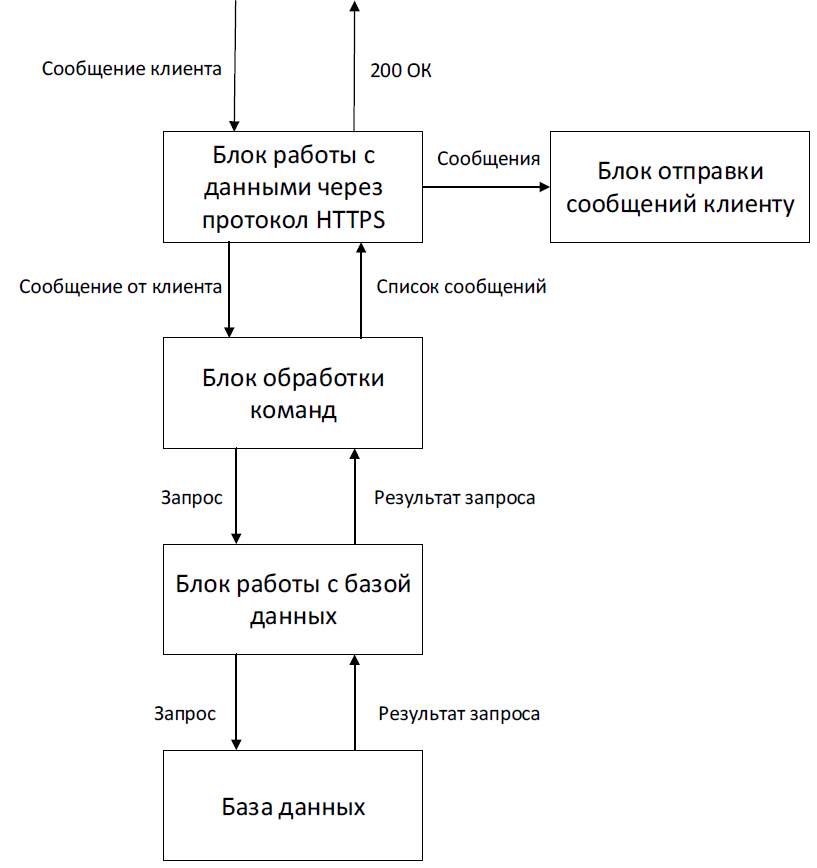
\includegraphics[scale=0.7]{structure_api.png}
	\caption{Схема взаимодействия блоков программного средства}
	\label{fig:design:architecture:structure_api}
\end{figure}

Опишем более подробно каждый из блоков.

\subsubsection{} Блок работы с данными через протокол HTTPS
\label{sec:design:server:api}

Отвечает за предоставление данных в определенном формате для клиентских приложений. Реализован в виде сервиса, основанного на webhook. Webhooks позволяют «сказать» серверам Telegram, что в случае, если появится сообщение для бота, отправлять их следует по ссылке, указанной в настройках конфигурации. Отпадает необходимость периодически опрашивать серверы самому, тем самым, снижается риск возникновения исключительных ситуаций в приложении. Однако, за это приходится платить установкой полноценного веб-сервера на машину, где предполагается запуск бота. Также, необходимо иметь SSL сертификат, так как webhooks в Telegram работают только по протоколу HTTPS.

Блок содержит в себе единственный контроллер с одним методом \emph{GetMessage}.

Метод принимает структуру \emph{Update}, которая содержит в себе все данные о сообщении, в том числе:

\begin{itemize}
	\item \emph{Message.Text} – текст сообщения.
	\item \emph{Message.From.FirstName} – имя пользователя.
	\item \emph{MessageFrom.LastName} – фамилия пользователя.
	\item \emph{MessageFrom.ChatId} – уникальный идентификатор чата.
\end{itemize}

В случае, если структура содержит в себе не сообщение, а, например, результат нажатия на кнопку \emph{InlineButton}, то свойство \emph{Message} будет иметь значение \emph{null}, а данные будут содержаться в свойстве \emph{CallbackQuery}.
Если структура не содержит ни текстового сообщения, ни результата нажатия на кнопку, сервером сразу же прерывается выполнение и отправляется ответ с кодом 200.

После получения нужных данных, управление передается в \emph{блок обработки команд}, который возвращает список структур \emph{HandlerServiceResult}, содержащих в себе следующие свойства:

\begin{itemize}
	\item \emph{StatusCode} – код результата.
	\item \emph{Message} – сообщение для отправки клиенту.
	\item \emph{Helper} – вспомогательное свойство, которое содержит список
вариантов ответов на вопросы, задаваемые ботом пользователю.
\end{itemize}

Структура содержит либо результат запроса пользователя, либо очередной вопрос, на который пользователю требуется ответить.
Далее управление передается блоку-обертке для отправки сообщения клиенту.
Также, в данном блоке настраиваются зависимости всего приложения, благодаря чему становится возможным использования принципа внедрения зависимостей. За это отвечают методы \emph{AddAppDependencies}, \emph{AddCommandHandler\linebreak Services}, \emph{AddDocumentServices}, а также \emph{AddTelegramBot}.

\subsubsection{} Блок обработки команд
\label{sec:design:server:framework}

Отвечает за выполнение бизнес правил приложения. Принимает данные от блока работы с данными через протокол HTTP и посылает их в блок работы с базой данных. Может быть размещен на отдельном сервере для увеличения производительности и снятия нагрузки с основных серверов.
Содержит структуры, перечисления и классы-помощники, необходимые для обработки команд.
Главный класс – \emph{CommandService}. Содержит структуру типа \emph{Dictionary<string, CommandHandlerDelegate>}, которая представляет собой словарь, ключом которого является название команды, значением – делегат, в который передается управление.
Инициализация структуры выполняется методом InitializeCommandHandlerDictionary, работа которого представлена в листинге ниже:

\lstset{style=sharpc}
\begin{lstlisting}
private void InitializeCommandHandlerDictionary()
{
	_commandHandlerDictionary = new Dictionary<string, CommandHandlerDelegate>
	{
		{"/help", _helpCommandHandlerService.Handle},
		{"/category", _categoryCommandHandlerService.Handle},
		{"/start", _startCommandHandlerService.Handle},
		{"/cancel", _cancelCommandHandlerService.Handle},
		{"/income", _operationCommandHandlerService.Handle },
		{"/expense", _operationCommandHandlerService.Handle },
		{"/stats", _statsCommandHandlerService.Handle }
	};
}
\end{lstlisting}

Главный метод класса – \emph{ExecuteCommand}. Он получает на вход сообщение пользователя, содержащее команду, либо ответ на вопрос. С помощью \emph{блока работы с базой данных} по свойству \emph{ChatId}, из базы данных извлекается текущий пользователь.
Модель пользователя содержит структуру \emph{Context}, с помощью которой реализуется модель контекста, когда пользователь вводит команду не целиком, а поэтапно, через вопросы бота. Структура представлена в листинге ниже:

\lstset{style=sharpc}
\begin{lstlisting}
public class Context
{
	public QuestionTree CurrentNode { get; set; }

	public string OperationId { get; set; }

	public string CategoryId { get; set; }

	public CategoryTypeEnum CategoryType { get; set; }
}
\end{lstlisting}

Свойство \emph{OperationId} указывает на идентификатор операции, с которой работает пользователь.
Свойство \emph{CategoryId} указывает на идентификатор категории, с которой работает пользователь.
Модель контекста содержит древовидную структуру \emph{QuestionTree}, каждый элемент которой представляет собой узел дерева, указывающий на детей данного узла, а также на элемент перечисления \emph{QuestionsEnum}. Структура QuestionTree описана в листинге ниже:

\lstset{style=sharpc}
\begin{lstlisting}
public class QuestionTree
{
	public List<QuestionTree> Children { get; set; }

	public QuestionsEnum Question { get; set; }
}
\end{lstlisting}

В перечислении \emph{QuestionsEnum} собраны все варианты вопросов, которые бот может задать пользователю для решения определенной задачи. Структура перечисления \emph{QuestionsEnum} описана в листинге ниже:

\lstset{style=sharpc}
\begin{lstlisting}
public enum QuestionsEnum
{
	None,
	CategoryAction,
	CategoryCurrency,
	CategoryType,
	CategorySupposedToSpentThisMonth,
	AddNewCategoryOrNot,
	CategoryName,
	EditCategory,
	DeleteCategory,
	AddCategory,
	OperationType,
	OperationCategory,
	OperationSum,
	OperationDate,
	ChooseCategoryToEdit,
	ChooseCategoryToDelete,
	StatsAction,
	StatsCategory,
	StatsCategoryDateRange
}
\end{lstlisting}

Если контекст пользователя не равен \emph{null}, это означает, что сообщение должно содержать ответ на текущий вопрос. С помощью методов расширения перечисления \emph{QuestionsEnum} определяется, является ли текущий вопрос вопросом по категориям, по статистике, либо по операциям. Управление передается в соответствующие методы классов-обработчиков.
В случае, если сообщение – команда, из структуры-словаря по ключу извлекается метод \emph{Handle} класса-обработчика данной команды, и управление передается классу-обработчику.
Классы-обработчики команд реализуют интерфейс \emph{IComandHandlerService}. Интерфейс описан в листинге ниже:

\lstset{style=sharpc}
\begin{lstlisting}
public interface ICommandHandlerService
{
	Task<List<HandlerServiceResult>> Handle(Message message);
}
\end{lstlisting}

Для генерации вопросов классы-обработчики используют сервис- \linebreak генератор вопросов \emph{QuestionService}. Сервис содержит структуру типа \linebreak \emph{Dictionary<string, QuestionsHandlerDelegate>}, которая представляет собой
15
словарь, ключом которого является одно из значений перечисления \linebreak \emph{QuestionsEnum}, значением – делегат, в который передается управление.
Инициализация структуры выполняется методом \linebreak \emph{InitializeQuestionBuilderDictionary}. Метод описан в листинге ниже:

\lstset{style=sharpc}
\begin{lstlisting}
private void InitializeQuestionBuilderDictionary()
{
	_questionsBuilderDictionary = new Dictionary<QuestionsEnum, QuestionsHandlerDelegate>
	{
		{QuestionsEnum.OperationCategory, BuildOperationCategoryQuestion},
		{QuestionsEnum.OperationDate, BuildOperationDateQuestion},
		{QuestionsEnum.OperationSum, BuildOperationSumQuestion},
		{QuestionsEnum.OperationType, BuildOperationTypeQuestion},
		{QuestionsEnum.CategoryAction, BuildCategoryActionQuestion },
		{QuestionsEnum.AddNewCategoryOrNot, BuildAddCategoryOrNotQuestion },
		{QuestionsEnum.CategoryName, BuildCategoryNameQuestion},
		{QuestionsEnum.ChooseCategoryToEdit, BuildCategoryToEditQuestion },
		{QuestionsEnum.ChooseCategoryToDelete, BuildCategoryToDeleteQuestion },
		{QuestionsEnum.CategoryType, BuildCategoryTypeQuestion },
		{QuestionsEnum.CategorySupposedToSpentThisMonth, CategorySupposedToSpentThisMonthQuestion },
		{QuestionsEnum.StatsAction, StatsActionQuestion },
		{QuestionsEnum.StatsCategory, StatsCategoryQuestion },
		{QuestionsEnum.StatsCategoryDateRange, StatsCategoryDateRangeQuestion },
		{QuestionsEnum.CategoryCurrency, CategoryCurrencyQuestion }
	};
}
\end{lstlisting}

Главный метод класса – \emph{BuildQuestion}. Из свойства \emph{Context} пользователя извлекается текущий узел дерева вопросов и используется в качестве ключа для выполнения метода генерации определенного вопроса.
Для генерации сообщений об ошибках либо результатах успешного выполнения команд используется сервис \emph{ResultService}.
Рассмотрим подробнее классы-обработчики.

\textbf{\emph{StartCommandHandlerService}}

Обработчик команды \emph{/start}. Выполняет проверку через \emph{блок работы с базой данных}, существует ли пользователь с данным \emph{ChatId} в базе данных. Если такого пользователя в базе данных не существует, он создается. Также, пользователю добавляются две стандартных категории Default Income Category и Default Expense Category. В ответ отправляет список команд, которые поддерживает бот.

\textbf{\emph{HelpCommandHandlerService}}

Обработчик команды \emph{/help}. Возвращает тот же ответ, что и \linebreak \emph{StartCommandHandlerService}.

\textbf{\emph{CancelCommandHandlerService}}

Обработчик команды \emph{/cancel}. С \emph{помощью блока работы с базой данных} извлекает текущего пользователя. Пользователь проверяется на наличие в контексте свойств \emph{OperationId} и \emph{CategoryId}. При наличии незавершенных категории либо операции, они удаляются из базы данных.

\textbf{\emph{СategoryCommandHandlerService}}

Обработчик команды \emph{/category}. Реализует логику приложения, отвечающую за категории. Содержит структуру типа \emph{Dictionary<string, \linebreak QuestionsHandlerDelegate>}, которая представляет собой словарь, ключом которого является название команды, значением – делегат, в который передается управление.
Инициализация структуры выполняется методом \linebreak \emph{InitializeQuestionsHandlerDictionary}. Метод описан в листинге ниже:

\lstset{style=sharpc}
\begin{lstlisting}
private void InitializeQuestionsHandlerDictionary()
{
	_questionsHandlerDictionary = new Dictionary<QuestionsEnum, QuestionsHandlerDelegate>
	{
		{QuestionsEnum.CategoryAction, ConfigureCategoryAction },
		{QuestionsEnum.CategorySupposedToSpentThisMonth, ConfigureCategorySupposedToSpentThisMonth },
		{QuestionsEnum.CategoryType, ConfigureCategoryType },
		{QuestionsEnum.AddNewCategoryOrNot, ConfigureCategoryCreating },
		{QuestionsEnum.CategoryName, ConfigureCategoryName},
		{QuestionsEnum.ChooseCategoryToDelete, ConfigureCategoryDelete },
		{QuestionsEnum.ChooseCategoryToEdit, ConfigureCategoryEdit },
		{QuestionsEnum.CategoryCurrency, ConfigureCategoryCurrency }
	};
}
\end{lstlisting}

Методы-значения отвечают за обработку ответов пользователя на вопросы бота, а также генерирование новых вопросов по необходимости.

Также содержит структуру типа \emph{QuestionTree}, представляющую собой дерево из вопросов пользователю. На рисунке~\ref{fig:design:server:category_service_scheme} представлена схема, изображающая структуру для категорий.

\begin{figure}[!h]
\centering
	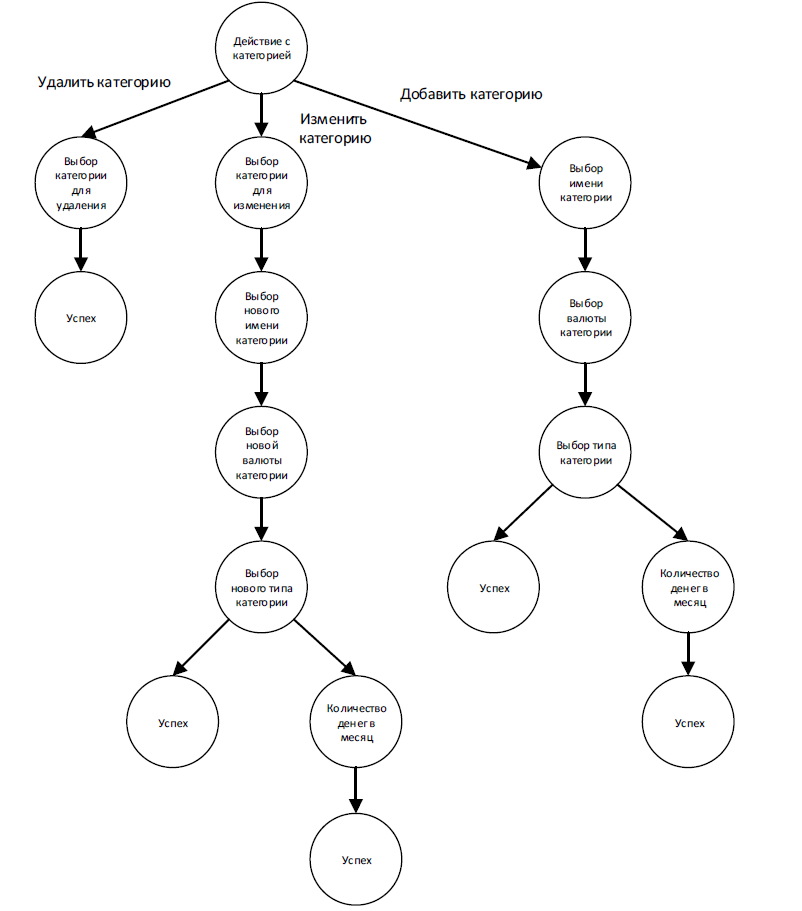
\includegraphics[scale=0.8]{category_service_scheme.png}
	\caption{Схема древовидной структуры вопросов по категориям}
	\label{fig:design:server:category_service_scheme}
\end{figure}

Пользователю на выбор даются 3 действия с категориями. При выборе удалить, предлагается список категорий для удаления. При выборе добавить, предлагается ввести имя категории, валюту, а также тип. Если тип категории – expense, то бот спустится ниже по дереву и задаст вопрос о том, сколько бы пользователь хотел тратить в месяц. Если категория – income, настройка категории будет считаться завершенной. При выборе изменить, предлагается список категорий для изменения. После выбора категории, запускается тот же сценарий, что и при добавлении.

Главный метод класса – \emph{Handle}. Принимает на вход структуру \emph{Message}. С помощью блока работы с базой данных извлекает текущего пользователя, а также категории данного пользователя. В случае отсутствия категорий, добавляет в древовидную структуру узел с вопросом, желает ли пользователь добавить категории, либо нет и возвращает вопрос. Если категории имеются, управление передается в генератор вопросов, который генерирует вопрос в соответствии с текущим узлом контекста пользователя.

Метод \emph{HandleCategoryQuestion} класса отвечает за обработку ответов
пользователей на вопросы бота. На вход принимает строку-ответ
пользователя, и структуру, описывающую самого пользователя.

С помощью структуры-словаря, по значению узла контекста
пользователя, управление передается в обработчик ответов.

\textbf{\emph{OperationCommandHandlerService}}

Обработчик команд /income и /expense. Реализует логику приложения,
отвечающую за операции. Содержит структуру типа \emph{Dictionary<string,
QuestionsHandlerDelegate>}, которая представляет собой словарь, ключом
которого является название команды, значением – делегат, в который
передается управление.

Инициализация структуры выполняется методом \linebreak
\emph{OperationCommandHandlerService}InitializeQuestionsHandlerDictionary. Метод описан в листинге ниже:

\lstset{style=sharpc}
\begin{lstlisting}
private void InitializeQuestionsHandlerDictionary()
{
	_questionsHandlerDictionary = new Dictionary<QuestionsEnum, QuestionsHandlerDelegate>
	{
		{QuestionsEnum.OperationDate, ConfigureOperationDate },
		{QuestionsEnum.OperationSum, ConfigureOperationSum },
		{QuestionsEnum.OperationCategory, ConfigureOperationCategory}
	};
}
\end{lstlisting}

Как и класс \emph{CategoryCommandHandlerService}, содержит структуру
\linebreak \emph{QuestionTree}, представляющую собой дерево из вопросов для пользователя. На рисунке~\ref{fig:design:server:operation_service_scheme} представлена схема данной структуры.

В начале выбирается категория для операции, далее запрашивается
сумма операции и дата. После введения всех данных, операция считается завершенной.

\begin{figure}[!h]
\centering
	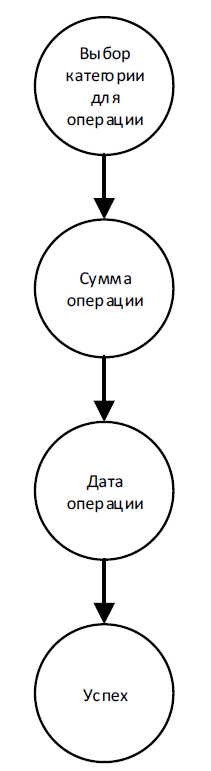
\includegraphics[scale=0.7]{operation_service_scheme.png}
	\caption{Схема древовидной структуры вопросов по категориям}
	\label{fig:design:server:operation_service_scheme}
\end{figure}

Главный метод класса – \emph{Handle}. С помощью блока работы с базой
данных извлекает текущего пользователя, а также в зависимости от команды \emph{/income} или \emph{/expense} устанавливает в контекст одно из значений перечисления \emph{CategoryTypeEnum}, описанного в листинге ниже:

\lstset{style=sharpc}
\begin{lstlisting}
public enum CategoryTypeEnum
{
	Income,
	Expense,
	None
}
\end{lstlisting}

Далее управление передается в метод \emph{ConfigureOperationType}, где с помощью блока работы с базой данных извлекаются все категории
пользователя данного типа. Если таких категорий не найдено, с помощью сервиса генерации сообщений об ошибках \emph{ResultService},генерируется сообщение о том, что таких категорий не найдено. Если категории найдены, в базу данных записывается операция, а управление передается генератору вопросов.

Метод \emph{HandleOperationQuestion} класса отвечает за обработку ответов пользователей на вопросы бота. На вход принимает строку-ответ пользователя, и структуру, описывающую самого пользователя.

\textbf{\emph{UnhandledMessageService}}

В случае, если бот не поддерживает данную команду, либо внутри программного средства было сгенерировано исключение, вызывается метод \emph{Handle} класса \emph{UnhandledMessageService}. В него передаются сведения о пользователе, сообщение пользователя, а также исключение. Обработчик упаковывает все данные в структуру \emph{UnhandledMessage} и, с помощью блока работы с базой данных, записывает её в базу. Структура \emph{UnhandledMessage} описана в листинге ниже:

\lstset{style=sharpc}
\begin{lstlisting}
public class UnhandledMessage : BaseModel
{
	public string Text { get; set; }

	public long ChatId { get; set; }

	public DateTime Created { get; set; }

	public Exception Exception { get; set; }
}
\end{lstlisting}

\textbf{\emph{StatsCommandHandlerService}}

Обработчик команды /stats. Реализует логику приложения, отвечающую за предоставление пользователю статистики по операциям. Содержит структуру типа \emph{Dictionary<string, QuestionsHandlerDelegate>}, которая представляет собой словарь, ключом которого является название команды, значением – делегат, в который передается управление.

Инициализация структуры выполняется методом \linebreak \emph{InitializeQuestionsHandlerDictionary}.

Как и в случае с классами \emph{CategoryCommandHandlerService} и \linebreak \emph{OperationCommandHandlerService}, данный класс имеет древовидную структуру, отвечающую за предоставление вопросов пользователю.

На рисунке~\ref{fig:design:server:stats_service_scheme} представлена схема этой структуры для класса \linebreak \emph{StatsCommandHandlerService}.

\begin{figure}[!h]
\centering
	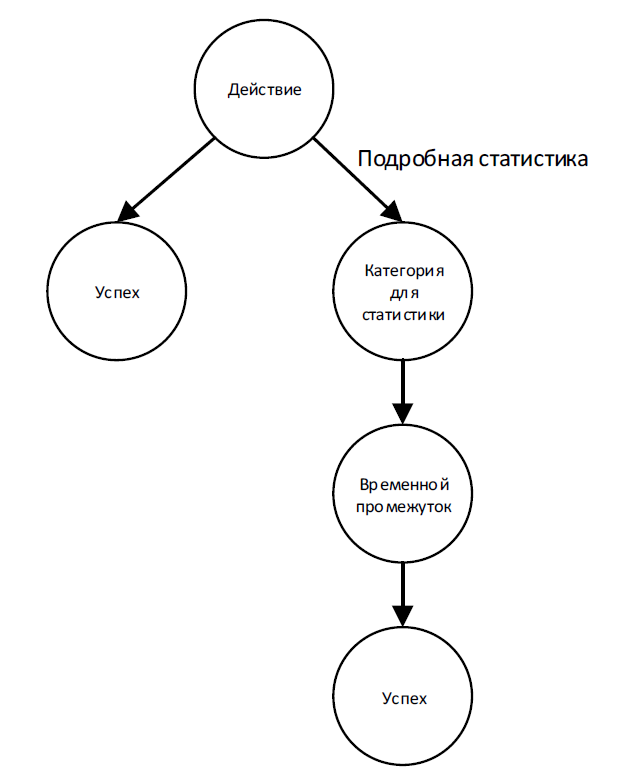
\includegraphics[scale=0.7]{stats_service_scheme.png}
	\caption{Схема древовидной структуры вопросов по статистике}
	\label{fig:design:server:stats_service_scheme}
\end{figure}

На выбор пользователю предлагаются 4 варианта: статистика по всем категориям, только \emph{income}, только \emph{expense}, либо подробная статистика. В случае выбора подробной статистики, бот запросит категорию для статистики, а также временной промежуток.

Для генерирования статистики используется сервис StatsService. В он себе содержит 2 перегрузки метода \emph{BuildStatistics}, описанные в листинге ниже:

\lstset{style=sharpc}
\begin{lstlisting}
public async Task<List<HandlerServiceResult>> BuildStatistics(Category category, DateTime? from = null, DateTime? to = null)

public async Task<List<HandlerServiceResult>> BuildStatistics(User user, CategoryTypeEnum type = CategoryTypeEnum.None)
\end{lstlisting}

Первая используется для генерации подробной статистики, вторая – для
генерации статистики для группы категорий.

\subsubsection{} Блок работы с базой данных
\label{sec:design:server:db}

Основная задача данного блока состоит в принятии запросов от блока
обработки команд для построения нужных моделей данных. Может быть
размещен на отдельном сервере для увеличения производительности и снятия нагрузки с основных серверов.

В приложении используются следующие модели данных:

\begin{itemize}
	\item Category – модель данных категории.
	\item Operation – модель данных операции.
	\item User – модель данных пользователя.
	\item UnhandledMessage – модель данных сообщения об ошибке.
	\item Chat – модель данных чата.
	\item Logs – модель данных логирования приложения.
	\item LogRequest – модель данных логирования запроса.
	\item LogResponse – модель данных логирования ответа.
	\item UserStatus – модель данных статуса пользователя.
	\item Context – модель данных контекста пользователя.
\end{itemize}

Данный блок был спроектирован с соблюдением паттерна «репозиторий», который делает структуру данного блока гибкой к изменениям. Если понадобится замена использующейся в проекте в данное время базы данных MongoDB, это можно будет сделать легко, заменив лишь класс с обращениями к драйверу базы данных.

Так как, на данный момент, в проекте используется MongoDB, то главным классом в блоке работы с базой данных является MongoService.

В нем происходит настройка и конфигурирование доступа к драйверу базы данных, а также предоставляется доступ к коллекциям.

Для каждой модели данных есть свой репозиторий:

\begin{itemize}
	\item CategoryDocumentService
	\item OperationDocumentService
	\item UnhandledMessageDocumentService
	\item UserDocumentService
	\item ChatDocumentService
	\item LogsDocumentService
	\item UserStatusesDocumentService
\end{itemize}

Все сервисы реализуют интерфейс IDocumentService<T>, описывающий базовые методы, которые должны быть реализованы каждым из сервисов. Структура интерфейса описана в листинге ниже:

\lstset{style=sharpc}
\begin{lstlisting}
public interface IDocumentService<T>
{
	Task InsertAsync(T item);

	Task UpdateAsync(T item);

	Task DeleteAsync(string id);

	Task<T> GetByIdAsync(string id);

	string GenerateNewId();
}
\end{lstlisting}

Также, все сервисы реализуют абстрактный класс \linebreak BaseDocumentService, в котором реализованы все базовые методы, нужные для работы приложения.

\subsubsection{} Описание классов и методов
\label{sec:design:server:methods}

В данном подразделе приведены сведения обо всех методах классов программного средства.

\begin{longtable}{|>{\raggedright}p{0.3\textwidth}|
		 >{\raggedright}p{0.3\textwidth}|
		 >{\raggedright\arraybackslash}p{0.32\textwidth}|} 
	\caption{Классы и методы блока работы через протокол HTTPS}
	\label{table:design:server:api}\\

	\hline
	\centering Класс & \centering Метод & \centering\arraybackslash Описание \endfirsthead

	\caption*{Продолжение таблицы \ref{table:design:server:api}}\\\hline
	\centering 1 & \centering 2 & \centering\arraybackslash 3 \\\hline \endhead

	\hline
	\centering 1 & \centering 2 & \centering\arraybackslash 3 \\
	\hline

	FinanceManager
BotController & GetMessage(Update update) & Получает структуру Update, извлекает из нее нужные данные, передает управление в блок обработки команд. После получения списка сообщений, передает управление в блок обработки сообщений. \\ \hline

	ControllerHelper & BuildKeyBoardMarkup(
List<string> options) & Строит и возвращает структуру InlineKeyBoardMarkup.
В качестве параметра принимает список строк, со значениями которых требуется построить виртуальные кнопки. В случае нечетного количества строк, последняя кнопка будет расположена на всю длину пространства.  \\ 

	& & Вызывается в случае, если для вопроса бота требуется виртуальные кнопки. \\ \hline

	BotExtensions & AddTelegramBot(this IServiceCollection services, IConfigurationRoot configuration) & Добавляет в контейнер Dependency Injection класс-обертку для посылки сообщений. \\ \hline

	BotExtensions & UseTelegramBot(this IApplicationBuilder app, string webhookPath) & Метод расширения IApplicationBuilder. Устанавливает боту адрес webhook. Запускает бот. \\ \hline

	Dependency
InjectionExtensions & AddAppDependencies
(this IServiceCollection) & Метод расширения IServiceCollection. Устанавливает зависимости для сервисов. \\ \hline

	Dependency
InjectionExtensions & AddCommandHandler
Services(this IServiceCollection) & Метод расширения IServiceCollection. Устанавливает зависимости сервисов-обработчиков команд. \\ \hline

Dependency
InjectionExtensions & AddDocumentServices
(this IServiceCollection) & Метод расширения IServiceCollection. Устанавливает зависимости сервисов-репозиториев. \\ \hline
\end{longtable}

\begin{longtable}{|>{\raggedright}p{0.3\textwidth}|
		 >{\raggedright}p{0.3\textwidth}|
		 >{\raggedright\arraybackslash}p{0.32\textwidth}|} 
	\caption{Классы и методы блока обработки команд}
	\label{table:design:server:framework}\\

	\hline
	\centering Класс & \centering Метод & \centering\arraybackslash Описание \endfirsthead

	\caption*{Продолжение таблицы \ref{table:design:server:framework}}\\\hline
	\centering 1 & \centering 2 & \centering\arraybackslash 3 \\\hline \endhead

	\hline
	\centering 1 & \centering 2 & \centering\arraybackslash 3 \\
	\hline

	CommandService & ExecuteCommand(string & Извлекает из базы \\ 

	& command, Message message) & данных пользователя, исходя из контекста пользователя, передает управление в классы-обработчики команд. В случае возникновения исключительной ситуации, вызывает обработчик UnhandledMessageService. \\ \hline

	CommandService & InitializeCommand
HandlerDictionary & Инициализирует словарь, ключом которого является команда, значением – делегат, в который передается управление. \\ \hline

	UnhandledMessage
Service & Handle(Message message, Exception exception) & Заполняет структуру UnhandledMessage данными из параметров и записывает её в базу. \\ \hline

CancelCommand
HandlerService & Handle(Message message) & Извлекает и базы данных текущего пользователя. Если он содержит ненулевой контекст, удаляет операцию, а также категорию из базы данных. Выставляет контекст пользователя в null. Сохраняет пользователя в базу. \\ \hline

HelpCommand
HandlerService & Handle(Message message) & Возвращает сообщение со списком команд, поддерживаемых ботом. \\

StartCommand
HandlerService & Handle(Message message) & Извлекает текущего пользователя из базы данных. Если пользователя с данным ChatId не существует, создает нового пользователя, а также 2 стандартных категории. Сохраняет пользователя в базу данных. \\ \hline

CategoryCommand
HandlerService & Handle(Message message) & Извлекает пользователя, а также его категории из базы данных. В случае, если категорий не существует, добавляет в древовидную структуру еще один узел и передает управление сервису построения вопросов. Если категории существуют, передает управление в сервис построения вопросов. \\ \hline

CategoryCommand
HandlerService & HandleCategoryQuestion
(string answer, User user) & Отвечает за обработку ответов пользователя на вопросы бота. Извлекает из контекста пользователя текущий узел и использует его как ключ для поиска метода, отвечающего за обработку, в словаре. Передает управление в метод-обработчик.
 \\

& & 
В случае, если в словаре не найден данный ключ, возвращает сообщение об ошибке. \\ \hline

CategoryCommand
HandlerService & InitializeQuestionTree() & Инициализирует древовидную структуру, использующуюся для реализации контекста. \\ \hline

CategoryCommand
HandlerService & InitializeQuestions
HandlerDictionaty & Инициализирует словарь, использующийся для обработки ответов пользователя. \\ \hline

CategoryCommand
HandlerService & ConfigureCategory
Action(string answer, User user) & Обрабатывает ответ пользователя на вопрос о действии с категориями. В случае, если ответ пустой, либо не содержит одного из нужных ответов, возвращается сообщение об ошибке.
В зависимости от ответа пользователя, проводятся соответствующие операции, а в контекст пользователя устанавливается узел-сын текущего узла. Управление передается в генератор вопросов. \\ \hline

CategoryCommand
HandlerService & ConfigureCategoryType
(string answer, User user) & Обрабатывает ответ пользователя на вопрос о типе категории. \\

& & Если ответ пустой, либо не содержит одного из нужных ответов, возвращается сообщение об ошибке. С помощью контекста пользователя, из базы извлекается категория. В случае, если тип категории является income, категория помечается как configured. Возвращается сообщение об успешном завершении настройки категории. В противном случае, в контекст устанавливается узел-сын текущего узла. Управление передается в генератор вопросов. \\ \hline

CategoryCommand
HandlerService & ConfigureCategory
Supposed
ToSpentThisMonth(
	string answer, User user) & Обрабатывает ответ пользователя на вопрос о сумме, которую он бы хотел тратить в месяц на эту категорию. В случае, если ответ пустой, либо не может быть представлен как тип данных long, возвращается сообщение об ошибке.
  \\ 

& & Из базы данных извлекается категория, в нее устанавливается сумма, описанная пользователем. Категория помечается как configured. Возвращается сообщение об успешном завершении настройки категории. \\ \hline

CategoryCommand
HandlerService & ConfigureCategory
Creating(string answer, User user) & Обрабатывает ответ пользователя на вопрос, требуется ли создание новой категории, или нет. В случае, если ответ пустой, либо не содержит нужного ответа, возвращается сообщение об ошибке. Если ответ да, в контекст устанавливается узел-сын текущего узла, управление передается в генератор вопросов. Если ответ нет, возвращается сообщение о том, что пользователь всегда может создать, удалить либо изменить категории с помощью соответствующей команды. \\

CategoryCommand
HandlerService & ConfigureCategoryName
(string answer, User user) & Обрабатывает ответ пользователя на просьбу ввести название категории.
Если ответ пустой, либо длиннее 30 символов, возвращаются соответствующие сообщения об ошибках. Если имя категории не уникально, возвращается сообщение об ошибке.
Категории устанавливается имя, в контекст устанавливается узел-сын текущего узла, управление передается в генератор вопросов. \\ \hline

CategoryCommand
HandlerService & ConfigureCategoryTo
Delete
(string answer, User user) & Обрабатывает ответ пользователя на вопрос, какую категорию следует удалить. Если ответ пустой, возвращается сообщение об ошибке. Если категории с таким именем не существует, возвращается сообщение об ошибке.
Категория удаляется, возвращается сообщение об успешном удалении категории. \\

CategoryCommand
HandlerService & ConfigureCategoryTo
Edit
(string answer, User user) & Обрабатывает ответ пользователя на вопрос, какую категорию следует изменить. Если ответ пустой, возвращается сообщение об ошибке. Если категории с таким именем не существует, возвращается сообщение об ошибке. В контекст пользователя помещается идентификатор категории, а также устанавливается узел-сын текущего узла. Управление передается в генератор вопросов. \\ \hline

CategoryCommand
HandlerService & ConfigureCategory
Currency
(string answer, User user) & Обрабатывает ответ пользователя на вопрос о валюте. Если ответ пустой, либо не содержит одного из вариантов ответа, возвращается сообщение об ошибке.
В категорию устанавливается валюта, в контекст устанавливается узел-сын текущего узла.
Управление передается в генератор вопросов. \\

Operation
Command
HandlerService & Handle(Message message) & Обрабатывает команды /income и /expense. Извлекает из базы данных текущего пользователя, устанавливает в контекст пользователя начальный узел структуры контекста. Управление передается в метод ConfigureOperationType. \\ \hline

Operation
Command
HandlerService & ConfigureOperationType
(CategoryTypeEnum type, User user) & Отвечает за обработку запроса пользователя. Если категорий с данным типом не существует, возвращается сообщение об ошибке.
В контекст устанавливается узел-сын текущего узла.
Управление передается в генератор вопросов. \\ \hline

Operation
Command
HandlerService & HandleOperation
Question
(string answer, User user) & Отвечает за обработку ответов пользователя. Используя контекст пользователя, передает управление в методы-обработчики.
В случае, если в словаре не найдено такого ключа, возвращается сообщение об ошибке. \\ 

Operation
Command
HandlerService & ConfigureOperation
Category
(string answer, User user) & Отвечает за обработку ответа пользователя на вопрос, какую категорию он хотел бы выбрать. Если ответ пустой, возвращается сообщение об ошибке. Если категории с таким именем не существует, возвращается сообщение об ошибке.
Категория добавляется в контекст, также в контекст устанавливается узел-сын текущего узла. Управление передается в генератор вопросов. \\ \hline

Operation
Command
HandlerService & ConfigureOperationSum
(string answer, User user) & Отвечает за обработку ответа пользователя на вопрос, на какую сумму совершается операция. Если ответ пустой, либо не может быть представлен в качестве типа decimal, возвращается сообщение об ошибке. Если тип категории – expense, и итоговые траты пользователя в этом месяце превысили теоретические, возвращается сообщение о превышении. \\ 

& & 
В контекст пользователя устанавливается узел-сын текущего узла. Управление передается в генератор вопросов. \\ \hline

Operation
Command
HandlerService & ConfigureOperationDate
(string answer, User user) & Отвечает за обработку ответа пользователя на вопрос о дате операции.
Если ответ пустой, возвращается сообщение об ошибке. Если сообщение не содержит приемлемого ответа, либо не может быть представлено в качестве типа DateTime, возвращается сообщение об ошибке.
В операцию записывается дата, и операция помечается как configured.
Возвращается сообщение об успешном завершении настройки операции. \\ \hline

Operation
Command
HandlerService & InitializeQuestionTree() & Инициализирует древовидную структуру данных, необходимую для контекста пользователя. \\ \hline

Operation
Command
HandlerService & InitializeQuestions
Handler
Dictionary() & Инициализирует структуру-словарь, ключами которой являются \\

& &  значения перечисления QuestionsEnum, значениями - делегаты. \\ \hline

StatsCommand
HandlerService & Handle(Message message) & Обрабатывает команду /stats. Извлекает из базы данных текущего пользователя, а также его категории. Если категорий не существует, возвращается сообщение об ошибке.
В контексте пользователя устанавливается узел контекста. Управление передается в генератор вопросов. \\ \hline

StatsCommand
HandlerService & HandleStatsQuestion
(string answer, User user) & Отвечает за обработку ответов пользователя на вопросы о статистике. С помощью контекста пользователя, управление передается в методы-обработчики. Если в словаре не найден такой ключ, возвращается сообщение об ошибке. \\ \hline

StatsCommand
HandlerService & ConfigureStatsAction
(string answer, User user) & Отвечает за обработку ответа пользователя на вопрос о действии со статистикой. Если ответ пустой, либо   \\ 

& & не содержит подходящего варианта, возвращается сообщение об ошибке. В зависимости от ответа пользователя, управление передается в сервис-генератор статистики. Если пользователь выбрал подробную статистику для одной категории, узел контекста принимает значение узла-сына, управление передается в генератор вопросов. \\ \hline

StatsCommand
HandlerService & ConfigureStatsCategory
(string answer, User user) & Отвечает за обработку ответа пользователя на вопрос о категории для статистики. Если ответ пустой, возвращается сообщение об ошибке. Если категория с таким именем у пользователя отсутствует, возвращается сообщение об ошибке. В контекст пользователя устанавливается категория, узел контекста принимает значение узла-сына. Управление передается в генератор вопросов.\\ \hline

\end{longtable}

\begin{longtable}{|>{\raggedright}p{0.3\textwidth}|
		 >{\raggedright}p{0.3\textwidth}|
		 >{\raggedright\arraybackslash}p{0.32\textwidth}|} 
	\caption{Классы и методы блока работы через протокол HTTPS}
	\label{table:design:server:db}\\

	\hline
	\centering Класс & \centering Метод & \centering\arraybackslash Описание \endfirsthead

	\caption*{Продолжение таблицы \ref{table:design:server:db}}\\\hline
	\centering 1 & \centering 2 & \centering\arraybackslash 3 \\\hline \endhead

	\hline
	\centering 1 & \centering 2 & \centering\arraybackslash 3 \\
	\hline

	BaseDocumentService & GenerateNewId() & Генерирует новый идентификатор. \\ \hline
	
	BaseDocumentService & InsertAsync(T document) & Асинхронно вставляет элемент в коллекцию. \\ \hline

	BaseDocumentService & UpdateAsync(T document) & Асинхронно обновляет элемент в коллекции. \\ \hline

	BaseDocumentService & DeleteAsync(string id) & Асинхронно удаляет элемент из коллекции. \\ \hline

	BaseDocumentService & GetByIdAsync(string id) & Асинхронно производит поиск и возвращает элемент из коллекции. \\ \hline

\end{longtable}